\documentclass{article}

\usepackage[final]{neurips_2018}

\usepackage[utf8]{inputenc}
\usepackage[T1]{fontenc}
\usepackage{hyperref}
\usepackage{url}
\usepackage{booktabs}
\usepackage{amsfonts}
\usepackage{nicefrac}
\usepackage{microtype}

\usepackage{color}
\usepackage{graphicx}
\usepackage{multirow}

\bibliographystyle{abbrvnat}

\title{Generating Music Using K-Means Clustering and Word2Vec Embeddings}

\author{
    William Lu \\
    60027133 \\
    \And
    Michael (Chih Hau) Hou \\
    22391156 \\
    \And
    Augustine Kwong \\
    35879155 \\
}

\begin{document}

\maketitle

\section{Introduction}

Algorithmic music generation is an enticing task. It is still unknown whether machine learning algorithms can achieve human-level creativity and understanding of musical structures such as melody, harmony, and form. Despite vast efforts, all current results to the best of our knowledge suffer from one or more of these limitations:

\begin{enumerate}
    \item The machine learning model involves deep belief networks or deep neural networks, including convolutional, recurrent, and long short-term memory architectures. Training these models requires lots of time and powerful hardware.
    \item The training data used must be in MIDI format. MIDI files of the complete works of a single composer are difficult to obtain whereas audio recordings are readily available.
    \item The generated music exhibits local structure in the form of semantically valid textures and chord progressions, but lacks global structure such as thematic development and formal coherence (\cite{music_generation_by_deep}). The generated music sounds reasonable in small segments, but lacks an obvious theme. A theme is defined in musicology as a short, recurring melody which is developed and transformed throughout the composition. Textures are defined as local note styles such as whether chords, scales, or thirds are utilized in a segment of music. Form is defined as the organizational pattern of a musical composition, given by the order in which themes are presented, developed, and recapitulated.
    \item In the case of the German \textit{Musikalisches Würfelspiel} ("musical dice game") generators, the generated music exhibits global structure, but only due to a human hard-coding all the possible correct choices for each generated measure (\cite{algorithmic_composition_computational_thinking}). To the best of our knowledge, no machine learning pipeline currently in existence learns semantic information in an unsupervised manner from a training corpus of audio data and then uses that semantic information to compose novel music.
\end{enumerate}

We tackle these four challenges in our project. We propose a machine learning pipeline which uses K-Means and Word2Vec to learn musical context and detect chunks of music that are semantically interchangeable. Our end-to-end pipeline receives training input and generates output in sound wave format.

We begin our paper with a discussion of common challenges in algorithmic music generation and a review of previous literature. We then describe our training dataset and our machine learning pipeline. We follow with an analysis of the behaviour of our pipeline and its generated music. We conclude with a summary of the limitations of our work and promising directions for future improvement.

\section{Challenges}

Music is generally stored in one of two data types. The first is MIDI, which is a computer-readable format representing sequences of notes and durations. Being deterministically parseable, MIDI representations are completely unambiguous and there are numerous libraries available for interpreting, editing, and playing back MIDIs. However, MIDI files for a complete compositional cycle, such as the set of all of Mozart's piano sonatas, are not readily available online. This poses challenges when crafting a training set consisting of stylistically similar music, preferably by one composer and in one genre.

Music is more commonly stored as raw sound wave data in formats such as WAV, FLAC, and MP3. Numerous instrumentalists have recorded complete compositional cycles on CD format. However, the analog nature of audio data makes it significantly harder to interpret and manipulate. Reconstructing sound data from computer-readable encodings and embeddings is difficult because slight modifications to the audio waveform can completely change the resulting sound. Audio recordings contain background noise and thus have more degrees of freedom than MIDI files of the same composition.

Another challenge is feature extraction for both MIDI and raw sound data. Musical structure is a mix of short-term, ``local'' dependencies and long-term, ``global'' dependencies. From a musicological perspective, important musical characteristics a composer may wish to consider include melody, phrasing, harmony, dynamics (loudness), tempo (speed), rhythm, texture, form, timbre, performing forces, and virtuosity (technical difficulty). Musical form is especially difficult to extract, because by definition it involves long-term dependencies. Harmonic progressions can be difficult to determine during cadenzas, which are long improvisatory sections containing embellishments in addition to the core harmony notes. Segmenting a melody line into phrases is ill-defined, since there are multiple feasible segmentations. Virtuosity is heavily dependent on whether a sequence of notes is comfortable and natural to play correctly. Simple metrics such as speed or note density are thus poor approximations of virtuosity.

Extracting key signatures, time signatures, and tempo markings from audio recordings is an open research problem, and new approaches are constantly discovered (\cite{end-to-end_musical_key_estimation}). Existing methods for separating melody and harmony lines are numerous (\cite{a_survey_of_melody}), but are not robust in contrapuntal sections where multiple variations of a melody are overlaid simultaneously. It is unclear how popular audio feature extractors, such as zero crossing rate and chroma frequencies, map to the aforementioned musical characteristics.

A third challenge is evaluation. Since music is an art form as opposed to a science, there is no objective standard by which the quality of a musical composition can be evaluated. It is hard to define what constitutes plagiarism and what merely constitutes inspiration or influence. Researchers typically conduct a user study where a third party provides their opinion, but this is infeasible for us due to the short time frame of our project. The lack of an objective metric makes supervised learning impossible. Thus, unsupervised learning models are the current \textit{de facto} standard for music generation.

\section{Related work}

Algorithmic music generation is a young field. Researchers have not yet reached a consensus on a standard machine learning technique for the task of generating music.

Previous research by Herremans and Chuan has investigated the usefulness of Word2Vec for learning musical context (\cite{modeling_musical_context_with}). The researchers use a dataset consisting of Beethoven's piano sonatas in MIDI format. Each major-key composition is transposed to C major, and each minor-key composition is transposed to A minor. They represent the music as a sequence of equal-length chunks and approximate each chunk by its closest chord. The researchers use these approximate chord sequences to train a Word2Vec model using skip-gram and negative sampling. They use t-SNE to visualize the learned chord embeddings. Chords that are tonally close on the circle of fifths appeared near each other on the t-SNE plot since they co-occur frequently in the training set. Chords that are tonally distant appeared in distinct clusters, demonstrating that Word2Vec is a reasonable model for learning harmonic progressions. In contrast to our project goal, the researchers do not attempt to leverage the chord embeddings for the purposes of music composition.

Recent research by Google DeepMind (\cite{the_challenge_of_realistic}) shows that autoencoders are successful in modeling raw audio data and are able to learn performance nuances present in music recordings that would be absent from MIDI files. The researchers' model is able to generate 10-second waveforms of piano timbre.

In 2016, Herremans designed an algorithm named \textit{MorpheuS} capable of generating music with long-term structure without using deep networks (\cite{morpheus_automatic_music_generation}). The algorithm takes a human-composed template as input and searches it for repeated form or tension profiles. It randomizes all the notes in the composition, then optimizes the notes to fit the learned tension profiles. MorpheuS generates music with harmonic and formal coherence but is unable to produce novel rhythms because it merely exchanges the notes in existing compositions.

Numerous approaches to music generation use deep networks (\cite{deepbach_a_steerable_model}, \cite{improved_music_feature_learning}, \cite{learning_features_from_music}). Researchers Huang and Wu use a recurrent neural network equipped with a long short-term memory architecture to build an end-to-end music generation model (\cite{deep_learning_for_music}). The authors note that training the model using stylistically homogeneous corpuses, such as those containing only music by a single composer, generated more aesthetically pleasing music. Kotecha and Young use two long short-term memory networks in a bi-axial configuration: one network learns melodic and harmonic traits and the other network learns patterns about note durations (\cite{generating_music_using_an}). The researchers explicitly mention the lack of long-term structure in the music generated by their model, and they note that adding a restricted Boltzmann machine that learns musical form to their configuration may address this deficiency. On the other hand, Briot and Pachet note in their deep learning review (\cite{music_generation_by_deep}) that restricted Boltzmann machines tend to plagiarize their training data. They suggest incorporating modified text plagiarism detection algorithms in pipelines involving restricted Boltzmann machines. Notably, probabilistic models and combinatorial optimization were popular techniques before the rise of deep learning (\cite{a_functional_taxonomy_of}).

\cite{a_functional_taxonomy_of} present a framework for categorizing the different methods used for extracting musical features from raw audio. The framework cites narrative, difficulty, melody, harmony, rhythm, and timbre as important musical characteristics. Abstract concepts such as narrative are difficult to concretely define: narrative might depend on chord progressions, recurring melodies, or other patterns. In sum, the definitions chosen by the machine learning engineer inevitably impose a subjective bias on the model.

\section{Training Dataset}

Our training corpus consists solely of audio recordings performed on modern grand pianos. We aim for stylistic homogeneity by including only piano solo, piano four-hands, or two-piano works of the Classical era (circa 1750-1825). Most of the compositions in our training corpus are multi-movement sonatas.

Table \ref{tab:training_corpus} summarizes the full list of recordings we used for training.

\begin{table}
    \centering
    \begin{tabular}{cccc}
        \toprule
        Composer & Compositions & Pianist & Format \\
        \toprule
        Ludwig van Beethoven & Piano Sonatas & Richard Goode & WAV \\
        \midrule
        \multirow{2}{*}{Muzio Clementi} & Piano Sonatas & \multirow{2}{*}{Howard Shelley} & WAV, FLAC, MP3 \\
        \cmidrule{2-2}
        \cmidrule{4-4}
        & Capriccios and Variations & & MP3 \\
        \midrule
        Franz Joseph Haydn & Piano Sonatas & John McCabe & WAV \\
        \midrule
        Johann Nepomuk Hummel & Piano Sonatas & Ian Hobson & WAV \\
        \midrule
        \multirow{3}{*}{Wolfgang Amadeus Mozart} & Piano Sonatas (Solo) & \multirow{3}{*}{Ingrid Haebler} & \multirow{3}{*}{MP3} \\
        \cmidrule{2-2}
        & Piano Sonatas (4-Hands) & & \\
        \cmidrule{2-2}
        & Piano Sonatas (2 Pianos) & & \\
        \midrule
        Franz Schubert & Piano Sonatas & Wilhelm Kempff & WAV \\
        \bottomrule
    \end{tabular}
    \caption{A list of the recordings in our training corpus.}
    \label{tab:training_corpus}
\end{table}

\section{Machine Learning Pipeline}

The source code of our machine learning pipeline is stored in a GitHub repository at \texttt{github.com/enchainingrealm/MusicGeneration}. Our pipeline consists of four modules:

\begin{enumerate}
    \item Feature extractor (\texttt{/src/vectorizer.py}, \texttt{/src/structs/*})
    \item K-Means (\texttt{/src/rescale.py}, \texttt{/src/kmeans.py})
    \item Word2Vec (\texttt{/src/word2vec.py})
    \item Music generator (\texttt{/src/generator/*})
\end{enumerate}

The feature extractor module takes the training corpus of raw sound data as its input. Using Python's \texttt{librosa} package, we load the sound files into memory at their original sampling rate. Due to the presence of frequent key changes in classical music and different movements of a single composition having different key signatures, we do not transpose all the files into the same key before running our feature extractor, in contrast to Herremans's previous work involving Word2Vec (\cite{modeling_musical_context_with}).

After loading the audio files, we segment each file into 1-second chunks. If the file length is not an exact integer number of seconds, the last chunk is naturally shorter than 1 second. For each chunk, we use \texttt{librosa}'s feature extraction methods to obtain a length-35 vector containing the following features of the chunk:

\begin{itemize}
    \item Zero crossing rate (scalar)
    \item Spectral centroid (scalar)
    \item Spectral rolloff (scalar)
    \item Mel-frequency cepstral coefficients (MFCCs) (length-20 vector)
    \item Chroma frequencies (length-12 vector)
\end{itemize}

The zero crossing rate is the number of times the audio signal changes from positive to negative, or vice-versa. It is an approximation of the percusiveness of the sound, and is theoretically useful for measuring the note density or musical texture of a chunk. The spectral centroid is the weighted mean of the frequencies present in the chunk's frequency spectrum. It is the center of mass of the frequency spectrum and models the perceived ``brightness'' of the sound, which is useful for differentiating between low and high tones. The spectral roll-off gives an alternative measure of timbre. The MFCCs encode common human speech patterns. This feature is included for completeness, but we do not anticipate its usefulness in encoding instrumental music. Lastly, the chroma frequencies encode information about the relative occurrence of each pitch class (C, C\#, D, D\#, etc.) in the chunk. We anticipate this feature to be useful in modeling key or chord progressions.

For each of these features besides the zero crossing rate, \texttt{librosa} produces values for each frame in the chunk. We average over all frames in the chunk to obtain the final feature values for the chunk.

The K-Means module takes the feature vectors produced by the feature extractor module as its input. We first rescale the MFCC and chroma frequency features: we multiply each of the MFCCs by $1 / \sqrt{20}$ and each of the chroma frequency coefficients by $1 / \sqrt{12}$. Intuitively, if two chunks have identical scaled features except for any one feature type having a difference of $1$ (in the scalar case) or $\vec{1}$ (in the vector case,) the two chunks have a Euclidean distance of $1$.

The K-Means module runs \texttt{scikit-learn}'s K-Means implementation on the scaled feature vectors. We cluster all the chunks in the training corpus into $1000$ clusters. Each cluster is meant to represent a single musical style that has appeared in a training composition. The members of a cluster are thus slight variations of the cluster's corresponding musical style.

The goal of the K-Means module is to create an approximate data representation that the Word2Vec module can operate on. The K-Means clusters are the ``words'' forming the Word2Vec module's vocabulary. The chunks in a cluster represent occurrences of the cluster's corresponding ``word'' in the training corpus. Since our K-Means module merely computes an approximate representation, it suffices to use only 4 random restarts. Each restart runs for a maximum of 300 iterations. We use $1731$ as our random seed for \texttt{scikit-learn}.

The Word2Vec module takes the K-Means module's cluster assignments as its input. For each composition in our training corpus, the Word2Vec module creates a ``sentence'' consisting of the cluster numbers of the chunks in the composition, in the chunks' original order. We then train \texttt{gensim}'s Word2Vec model on the ``sentences'', using 50-dimensional word vectors, negative sampling, window length 5, and a random seed of $1731$.

Our music generator module takes a template composition as input and splits it into its constituent template chunks. We generate a new composition by replacing each template chunk $x$ with another similar chunk $\tilde{x}$ in the training corpus, according to a distance metric. Our generator supports four different metrics. Denote the cluster of $x$ as $c$.

\begin{itemize}
    \item The \texttt{kmeans\_random\_generator.py} generator replaces each $x$ with a random $\tilde{x}$ in $c$.
    \item The \texttt{kmeans\_nearest\_generator.py} generator replaces each $x$ with the nearest $\tilde{x}$ (in terms of Euclidean distance between $x$ and $\tilde{x}$'s scaled feature vectors) in $c$ such that $\tilde{x} \neq x$.
    \item The \texttt{word2vec\_cosine\_generator.py} generator finds the nearest cluster $\tilde{c}$ to $c$ (in terms of cosine similarity between the Word2Vec cluster embedding vectors) such that $\tilde{c} \neq c$. This generator replaces $x$ with the chunk $\tilde{x}$ in $\tilde{c}$ that is nearest (in terms of scaled feature vectors) to $x$.
    \item The \texttt{word2vec\_euclidean\_generator.py} generator uses Euclidean distance between embedding vectors instead of cosine similarity. Thus, this generator also accounts for the relative frequencies of cluster occurrences.
\end{itemize}

\section{Results and Analysis}

Our training corpus contains 209492 chunks in total. The number of chunks from each composer are summarized in Table \ref{tab:composer_chunks}. We note that Clementi is the most prolific composer in our corpus, and Hummel is the least prolific.

\begin{table}
    \centering
    \begin{tabular}{ccc}
        \toprule
        Composer & \# of chunks & \% of the training corpus \\
        \toprule
        Ludwig van Beethoven & 36554 & 17.45\% \\
        \midrule
        Muzio Clementi & 56364 & 26.91\% \\
        \midrule
        Franz Joseph Haydn & 52521 & 25.07\% \\
        \midrule
        Johann Nepomuk Hummel & 8884 & 4.24\% \\
        \midrule
        Wolfgang Amadeus Mozart & 27516 & 13.13\% \\
        \midrule
        Franz Schubert & 27653 & 13.20\% \\
        \bottomrule
    \end{tabular}
    \caption{The number of chunks, and the percentage of our entire training corpus, composed by each composer.}
    \label{tab:composer_chunks}
\end{table}

The distributions of the scalar features extracted from the training chunks are displayed in Figures \ref{fig:zero_crossing_rate_distribution}, \ref{fig:spectral_centroid_distribution}, and \ref{fig:spectral_rolloff_distribution}. Summary statistics are presented in Table \ref{tab:feature_summary}. All three scalar features follow an approximately normal distribution, although each distribution has a long right tail. The zero crossing rate distribution is especially skewed with a skewness of $13.70$. The spectral rolloff distribution has a less sharp peak than the other two distributions, with a kurtosis of only $37.87$.

\begin{figure}
    \centering
    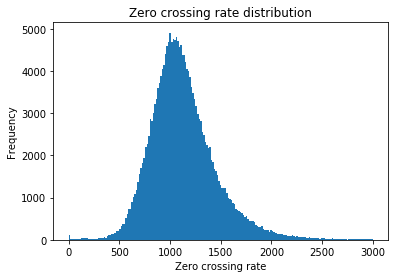
\includegraphics[width=0.67 \linewidth]{zero_crossing_rate_distribution.png}
    \caption{Histogram of zero crossing rate value distribution over the training chunks.}
    \label{fig:zero_crossing_rate_distribution}
\end{figure}

\begin{figure}
    \centering
    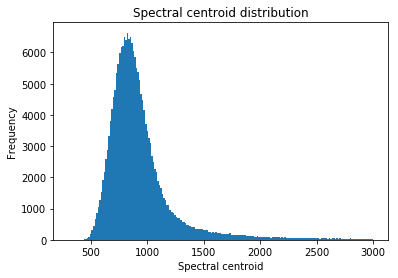
\includegraphics[width=0.67 \linewidth]{spectral_centroid_distribution.png}
    \caption{Histogram of spectral centroid value distribution over the training chunks.}
    \label{fig:spectral_centroid_distribution}
\end{figure}

\begin{figure}
    \centering
    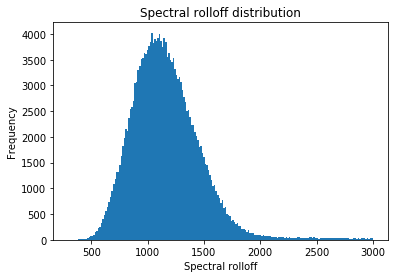
\includegraphics[width=0.67 \linewidth]{spectral_rolloff_distribution.png}
    \caption{Histogram of spectral rolloff value distribution over the training chunks.}
    \label{fig:spectral_rolloff_distribution}
\end{figure}

\begin{table}
    \centering
    \begin{tabular}{ccccccc}
        \toprule
        Feature & Mean & Std & Min & Max & Skewness & Kurtosis \\
        \toprule
        Zero crossing rate & 1222.34 & 1127.38 & 0 & 38966 & 13.70 & 254.06 \\
        \midrule
        Spectral centroid & 1062.44 & 944.20 & 0.00 & 18271.98 & 7.08 & 63.57 \\
        \midrule
        Spectral rolloff & 1584.54 & 2228.64 & 0.00 & 21676.76 & 5.96 & 37.87 \\
        \bottomrule
    \end{tabular}
    \caption{Summary statistics for the distributions of the three scalar features.}
    \label{tab:feature_summary}
\end{table}

At \texttt{drive.google.com/open?id=1EO3gyb2ikc6Mdax4bW3eOvY2yK40K4\_a}, we present the audio generated by our pipeline. We save waveforms containing all the chunks assigned by K-Means to clusters 0 through 9 in \texttt{/data/output/ClusterGenerator/}. Cluster 0 contains rapid, medium-quiet notes reminiscent of Alberti-bass textures. Clusters 1, 3, 5, and 9 contain quiet or silent chunks, although clusters 1 and 5 contain a few louder moments. Clusters 2, 7, and 8 contain complete silence. Cluster 4 contains harsh accented and percussive tones. Cluster 6 lacks a defining characteristic, although all its chunks are medium in volume.

Generally, clusters containing many chunks also contain louder chunks. Figure \ref{fig:chunks_per_cluster_distribution} plots the size (number of chunks in cluster) distribution of the clusters. The majority of the clusters contain less than 100 chunks. The quiet or silent chunks are distributed throughout the numerous small clusters. The loud moments in clusters 1 and 5 belong to mostly-quiet chunks which were clustered alongside completely quiet chunks.

\begin{figure}
    \centering
    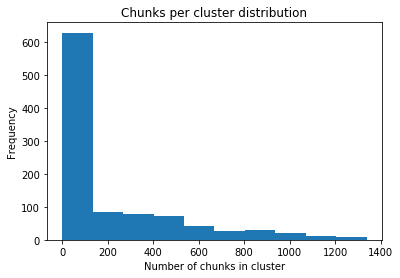
\includegraphics[width=0.67 \linewidth]{chunks_per_cluster_distribution.png}
    \caption{Size (number of chunks in cluster) distribution for K-Means clusters.}
    \label{fig:chunks_per_cluster_distribution}
\end{figure}

To visualize the geometry of our learned K-Means clusters, we plot the cluster means using principal component analysis with 2 principal components in Figure \ref{fig:kmeans_pca}. Larger dots indicate clusters that contain more chunks. Notably, most of the clusters containing high numbers of chunks are located at the bottom left corner of the plot. That, in addition to most of the variance in the cluster means being explainable with one principal component, hints at our feature extractor module failing to truly separate different musical keys, chords, and textures. The current clustering merely places the clusters with no audio or quiet audio in the right side of the plot, away from the clusters containing louder audio at the bottom left. It is likely that the first principal component is a measure of audio loudness.

\begin{figure}
    \centering
    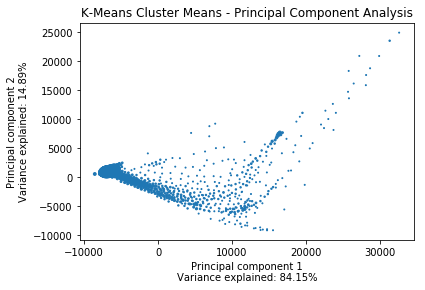
\includegraphics[width=0.67 \linewidth]{kmeans_pca.png}
    \caption{Principal Component Analysis plot of K-Means cluster means.}
    \label{fig:kmeans_pca}
\end{figure}

We visualize our Word2Vec cluster embeddings using principal component analysis in Figure \ref{fig:word2vec_pca}. The smaller clusters and larger clusters are clearly separated in the plot. Recalling our previous observation that smaller clusters contain quieter chunks, this is consistent with the assumption that most music does not contain sudden dynamic changes and can thus be separated into ``loud'' and ``quiet'' contexts.

\begin{figure}
    \centering
    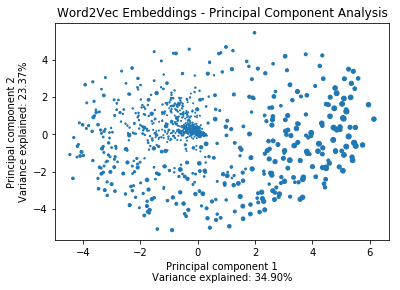
\includegraphics[width=0.67 \linewidth]{word2vec_pca.png}
    \caption{Principal Component Analysis plot of Word2Vec embeddings.}
    \label{fig:word2vec_pca}
\end{figure}

Due to the lack of a universal quantitative metric for music quality, we evaluate our music generator module purely by listening to the generated audio saved at \texttt{/data/output/}. For each of the four distance metrics supported by the music generator module, we try using the compositions listed in Table \ref{tab:template_compositions} as template compositions. In most cases, the generated music is similar to the template in terms of loudness patterns. However, the boundaries between adjacent chunks in the generated music are clearly audible, and there are no notable melodic or harmonic progressions. This is consistent with the principal component analysis visualizations suggesting that our feature extractor module successfully captures percusiveness and loudness, but not pitch, harmony, or key.

\begin{table}
    \centering
    \begin{tabular}{cc}
        \toprule
        Composer & Composition \\
        \toprule
        Ludwig van Beethoven & Piano Sonata No. 21 Op. 53 in C Major Mvt. 1 \\
        \midrule
        Muzio Clementi & Piano Sonata Op. 25 No. 5 in F-Sharp Minor Mvt. 3 \\
        \midrule
        Franz Joseph Haydn & Piano Sonata No. 60 Hob. XVI:50 in C Major Mvt. 1 \\
        \midrule
        Johann Nepomuk Hummel & Piano Sonata No. 5 Op. 81 in F-Sharp Minor Mvt. 1 \\
        \midrule
        Wolfgang Amadeus Mozart & Piano Sonata KV 448 (375a) in D Major Mvt. 1 \\
        \midrule
        Franz Schubert & Piano Sonata No. 21 D. 960 in B-Flat Major Mvt. 1 \\
        \bottomrule
    \end{tabular}
    \caption{Template compositions used to evaluate the music generator module.}
    \label{tab:template_compositions}
\end{table}

\section{Limitations and Future Work}

The most significant limitation of our pipeline is its inability to produce completely novel melodies from scratch. Instead, it simply rearranges pre-existing material in a contextually feasible manner. Overcoming the challenge of composing truly original music with original stylistic traits will likely require a departure from purely machine learning-based approaches, which naturally seek to replicate previously human-composed musical styles found in the training corpus. A model capable of composing original music would likely use insights from symbolic programming for understanding music-theoretic compositional heuristics. Computational optimization algorithms would also be a likely component of such a model, for quantifying and maximizing the quality of a generated composition. Lastly, such a model would need to be trained on a corpus of MIDI files (at least initially) as opposed to audio files due to the difficulty of synthesizing convincing musical audio data from scratch.

Frequently, the chunks generated by our pipeline are wildly different from the original template chunks. The problematic components of our pipeline are likely not the machine learning models \textit{per se}. Rather, our feature representation fails to capture all the musical characteristics required. Notably, the use of the chroma frequency features does not guarantee that the generated chunks are based on the same chords as the template chunks, although chroma frequency theoretically represents the tonal center of a chunk. Future work may focus on designing a better key or chord extractor.

Adjacent chunks generated by our pipeline do not transition smoothly. One can hear obvious gaps and discontinuities at the chunk borders in the generated audio. Adding a custom convolution that heavily weighs data close to the boundaries of a chunk into our feature representation may alleviate this problem. More intelligent chunking criteria that takes into account musical phrasing, measures, or tempo may produce more reasonable chunks.

Lastly, one possible extension to our pipeline that could improve global musical structure is to integrate a hidden Markov-model logic into our generators. With this extension, our generator has two modes: a ``create'' mode and a ``repeat'' mode. The generator would routinely transition between these modes based on its transition probabilities. In the ``create'' mode, the generator would retain its current behaviour. In the ``repeat'' mode, the generator would begin to copy previously generated material. Enforcing repetition of material appearing earlier in the generated composition gives a primitive illusion of form. However, copying previous parts of the generated composition verbatim completely disregards key changes and other variational techniques that enhance repetitions in classical-era music.

\section{Conclusion}

In this paper, we described a novel machine learning architecture that uses K-Means and Word2Vec for generating music based on a corpus of training data in sound wave format. The generated samples sound superficially meaningless, although a more involved analysis using principal components demonstrated that the machine learning algorithms in our pipeline are indeed finding reasonable clusters and embeddings. Further improving our pipeline requires enhancing our feature extraction methodology to better capture tonality and designing a method to ensure that adjacent chunks in the generated audio transition smoothly.

\bibliography{bibliography}
\end{document}
